To quantify the systematics of lens modeling for clusters typically found in surveys, we need to take similar approaches as we have done in Chap~\ref{chap:ares_systematics} and look to simulations. In this chapter, I will present an example of what such an analysis might look like.

\section{The simulated cluster}

For this analysis, I will be using a cluster created in an N-body simulation using the Hardware/Hybrid Accelerated Cosmology Code \citep[HACC; ][]{Habib:2016cy}. This code includes both baryons and dark matter; however only accounts for gravitational interactions. Therefore, any feedback mechanisms as the galaxies form are ignore as well as ram pressure stripping which can truncate galaxy halos as they fall into the cluster and pass through the hot intercluster medium. \citet{Li:2016ek} searched the resulting clusters for those which produce significant critical curves at $z=2$, and using a Pipeline for Images of Cosmological Strong lensing (PICS), have generated many realistic images of strong lensing systems. For this particular exercise, I have selected one of these lensing systems, a seemingly-relaxed cluster at $z=0.349$, shown in Figure~\ref{chap6:fig:cluster}.

\begin{figure}
\centering
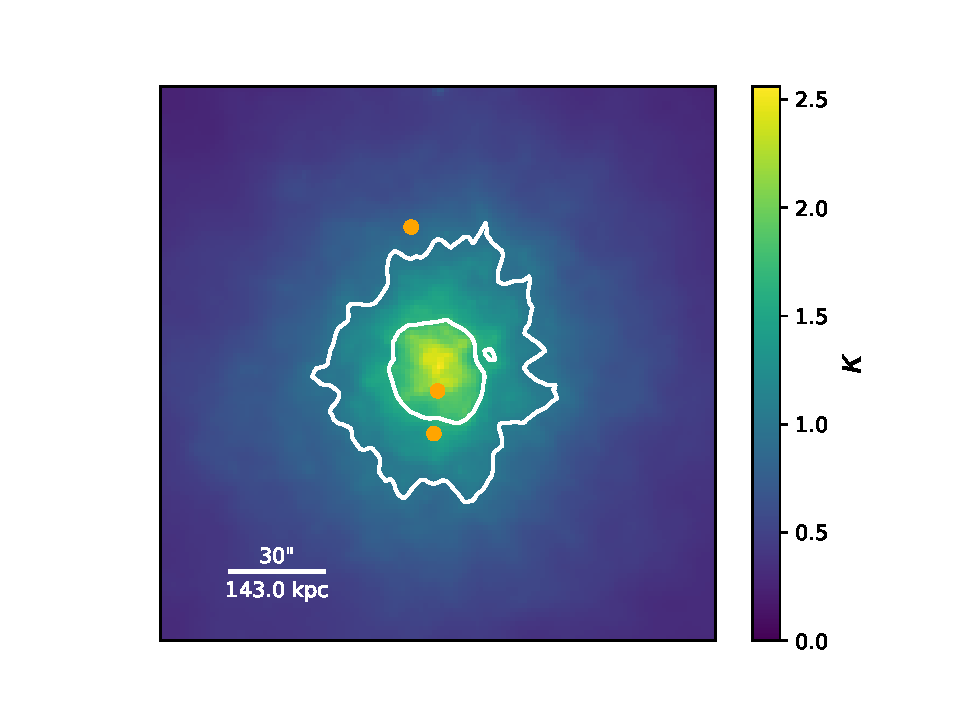
\includegraphics[width=\textwidth,trim={0 33pt 0 40pt},clip]{Chap6/cluster.pdf}
\caption[Simulated cluster from created using HACC]{Simulated cluster at $z=0.349$ created using the HACC code \citep{Habib:2016cy}. Shown $\kappa=\Sigma/\Sigma_\mathrm{crit}$, the surface mass density in units of the critical density for a source at $z=1.9615$. The white line is the critical curve for $z=1.9615$. Shown is example image configuration for a source at $z=1.9615$.}
\label{chap6:fig:cluster}
\end{figure}

\section{Methods}

Using the derived deflection fields for the mass distribution of this cluster, I have produced hundreds of simulated multiple image systems with source redshifts from $z=1-6$, placed at random positions behind the lens. From these systems, I have selected 100 subsets of five image configurations to create lens models. This lens models were created using \texttt{LENSTOOL} and are very simple: they consists of a single Pseudo-Isothermal Elliptical Mass Distribution with six free parameters: $x,y$ position, fiducial velocity dispersion, core radius, ellipticity, and position angle. Each model uses the same distribution of priors for this halo. Since the baryons in the simulation are not tracked, I do not have the tools to map the observed light distribution with halos, so for now, the lens models consist only of the primary dark matter halo without satellite galaxy halos. For speed, each model was produced using source plane minimization.

Once each model was created using five image systems all with known redshifts, another model was created from that model, but with either removing one image or replacing the known redshift with an unknown redshift as a free parameter in the model. After creating this new model, another was created from that one using the same process as before and so on, until the number of constraints was insufficient for the number of free parameters in the model. This process led to a total of 1024 models with varying number of sources, number of images, and number of known redshifts.

\section{Results}

There are several relationships between model inputs I could explore, but to keep things short, I will compare the systematic errors on both the mass and magnification as functions of only the number of spectroscopic redshifts in a model. The top of Figure~\ref{chap6:fig:systematic_errors} shows the distribution of derived masses within a radius of 100~kpc of the cluster center as a function of number of known (``spectroscopic") redshifts. Also shown in this figure is the true mass from the simulation. To understand the effects of systematics on the magnification, we track the magnification of a single image from a source $z=1.9615$, the top image shown in Figure~\ref{chap6:fig:cluster}. The bottom of Figure~\ref{chap6:fig:systematic_errors} shows the distribution of magnifications of this image as a function of number of spectroscopic redshifts.

\begin{figure}
\centering
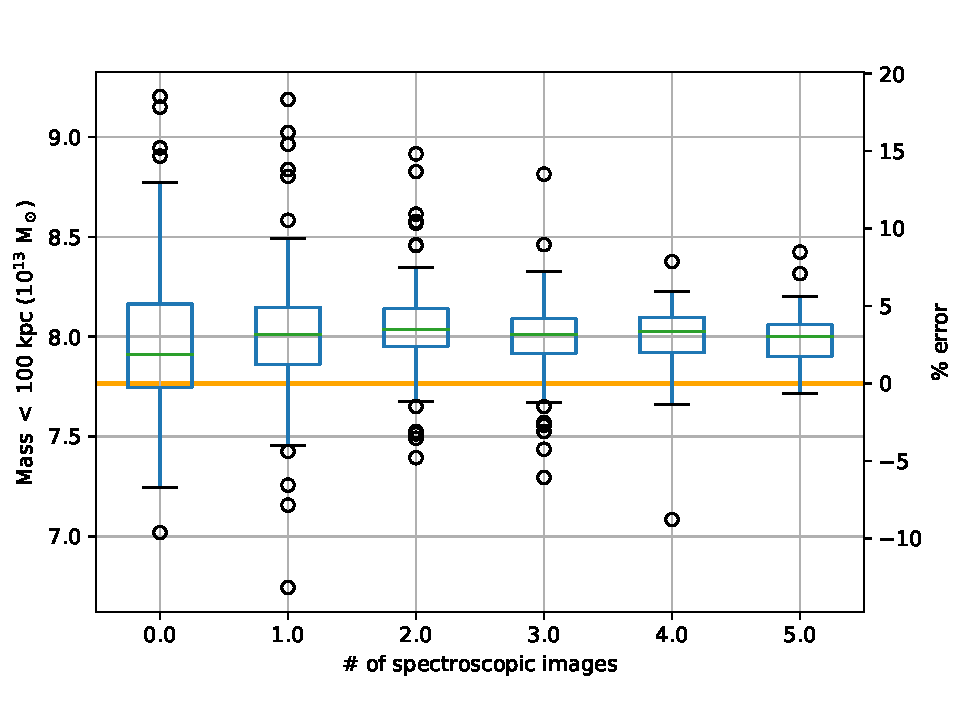
\includegraphics[width=0.8\textwidth]{Chap6/mass.pdf}
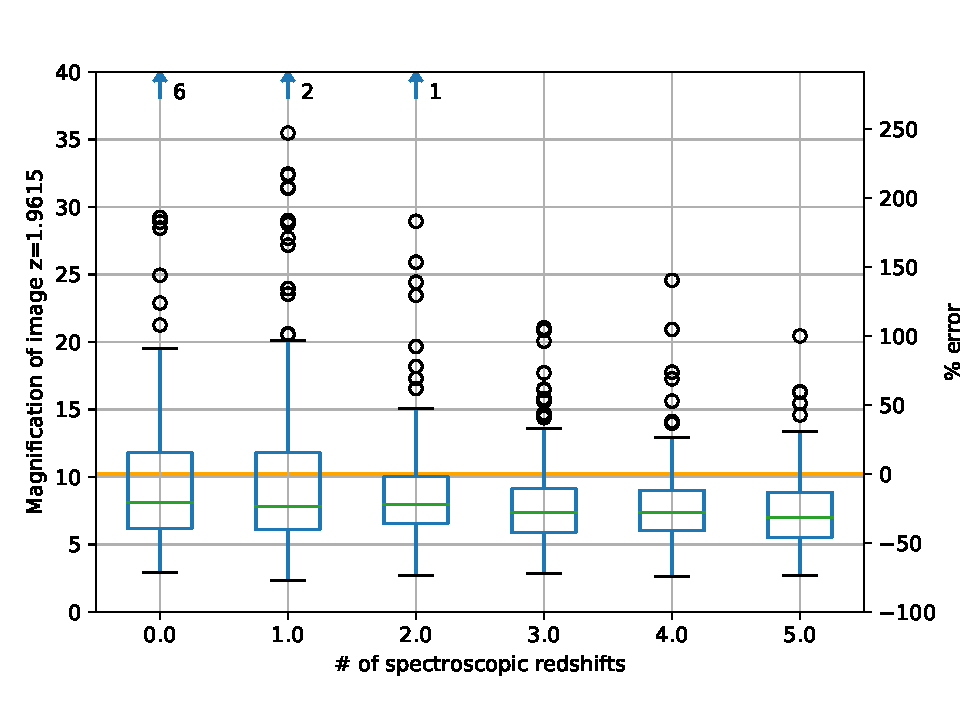
\includegraphics[width=0.8\textwidth]{Chap6/mag.pdf}
\caption[Masses and magnifications of the simulated cluster derived from 1024 lens models]{(Top) The distribution of derived mass within 100~kpc of the simulated cluster core from 1024 lens models with varying numbers of known (``spectroscopic") redshifts. (Bottom) The distribution of derived magnifications for the top image in Figure~\ref{chap6:fig:cluster} at $z=1.9615$. (Both) The orange horizontal lines indicate the values calculated from the true mass and magnification of the simulated cluster.}
\label{chap6:fig:systematic_errors}
\end{figure}

\section{Discussion}

For both the mass and magnification, we see that after adding two spectroscopic redshifts to a model, the systematic errors begin to reach a threshold of $\sim1\%$ and $\sim10\%$, respectively. However, when comparing to the true values computing from the simulation, we see that the derived values obtained are biased by $+3\%$ in mass and $-30\%$ in magnification. 

These offsets may be a result of having too simple of a lens model. Since we are not accounting for the substructure, we are missing mass from the brightest cluster galaxy as well as other galaxies near the core of the cluster. In order to replicate the lensing in the core of the cluster, the main halo may have to have parameters which increase the overall mass in the center of the cluster, which might account for an overall increase in the mass distribution within 100~kpc. Mass might also be missing near this particular image which may influence the local lensing potential and thus influence the deflection of this image significantly compared to the contribution by the overall deflection from the main cluster halo. This explains why the magnification might be lower than the true cluster, which has the extra mass to boost the magnification to higher values.

Clearly this analysis is very shallow and requires several more aspects that are not investigated here:

\begin{itemize}
\item Baryons: Simulations need to account for the distribution of baryons as well as the physics beyond gravity which can influence their distributions. Since the lens modeling method used here assumes that light traces mass, we need to know where the baryons are to infer where the mass is and to test how well this assumption works when tested against the simulation.
\item Image configurations: Certain image configurations may allow for better constraints in certain parts of the image plane. For example: using radial images allows for a better constraint on the innermost part of the mass profile. Similarly, if images are located very close together in the image plane, only the parts of the image plane near those images will be better constrained than others. In this analysis, we looked at the magnification of a single image; however, we have not included information related to the other image systems from which those models were created.
\item Other types of clusters: Some clusters can produce more elongated critical curves as a result of their shapes or because they are in the process of merging with another cluster. These effects can produce different image configurations which could cause different systematic errors that we may or may not see in the cluster we have chosen.
\item Redshift distribution of images: Since the location of the Einstein radius depends on the redshift of the background source, the mass will be better constrained the radii where the images are located. Similarly, the location of the critical curves will be best constrained for redshifts of images used in the models. 
\end{itemize}

More in-depth analyses of the systematics of lensing clusters with few constraints taking into account these aspects will be explored further in the future.
